\chapter{Use Cases}
In this section, we will describe potential uses for our system. Backup systems have a fairily specific set of use cases, as seen in the following figure.

\begin{figure}[h]
\centering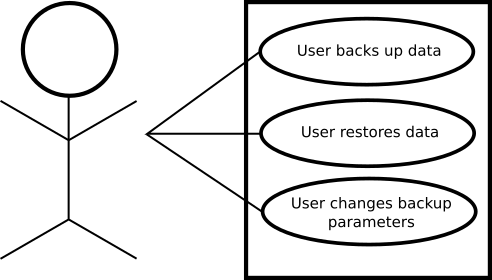
\includegraphics[scale=0.5]{images/senior-design-user-model.png}
\caption{Use Cases}
\end{figure}

This backup product has a very specific set of use cases. Typical user sessions are listed below.

\section{Backing Up}
\begin{itemize}
	\item Principle Actor: User
	\item Pre-conditions: 
		\begin{itemize}
			\item User has installed the backup client 
		\end{itemize}
	\item Post-condition:
			\begin{itemize}
				\item User has backed up desired files
			\end{itemize}
	\item Steps:
		\begin{enumerate}
			\item User opens configuration application
			\item User specifies which files to back up and schedules the backup
			\item The storage device backs up the indicated files at the specified time
		\end{enumerate}
\end{itemize}
\section{Restoring}
\begin{itemize}
	\item Principle Actor: User
	\item Pre-conditions: 
		\begin{itemize}
			\item User has installed the backup client
		\end{itemize}
	\item Post-condition:
			\begin{itemize}
				\item User has restored the desired files
			\end{itemize}
	\item Steps:
		\begin{enumerate}
			\item User opens configuration application
			\item User indicates which files to be restored
			\item User selects the restore action
			\item The storage device has written the desired files to the users computer
		\end{enumerate}
\end{itemize}
